\chapter{State of the Art}\label{sec:state-of-the-art}
Dieser Teil der Arbeit befasst sich mit vergleichbaren Serious Games im Schlaganfallrehabiliationbereich. Es wird kurz erklärt, wie die Spiele funktionieren und welchen Funktionsumfang diese besitzen. Zudem wird darauf eingegangen, ob und welche Daten durch die Systeme aufgezeichnet werden. Am Ende werden die unterschiedlichen Lösungen anhand von einigen Kriterien verglichen.

\section{Rehab@Home}\label{sec:rehab@home}
\enquote{Rehab@Home} ist ein Projekt für Schlaganfallpatient/innen, welches von der Europäischen Union (EU) finanziert wurde. Die Unternehmung lief von 2012 bis 2015 mit einem Budget von rund 3,2 Millionen Euro. Die Forschung bezieht sich auf die obere Körperhälfte, speziell die Bewegung der Arme und Handgelenke. Das Ziel des Projekts war es, dass ein IT-Gerät entwickelt wird, welches den Patient/innen erlaubt ihre Rehabilitationsübungen zu Hause zu machen. Das Gerät bietet eine Reihe von personalisierten Serious Games für jede/n Patient/in. Die Spiele werden für jede/n Patient/in durch den/die Ärzt/in ausgewählt und auf die Bedürfnisse und Fähigkeiten angepasst. Der/Die Spieler/in sammelt beim Spielen Punkte, die mit Freund/innen oder Familienmitgliedern verglichen werden können. \enquote{Rehab@Home} steht für mehrere Endgeräte zur Verfügung (Wii, Kinect, Stifteo Cubes). Das Projekt soll dazu beitragen, dass die Motivation der Patient/innen gesteigert wird und so die Übungen regelmäßiger durchgeführt werden. Ärzt/innen haben zusätzlich die Möglichkeit, den Therapieerfolg der Patient/innen zu Hause mitzuverfolgen. Das System bietet eine Auswahl aus sechs Spielen (siehe Abbildung \ref{fig:rehab@home:2016}), die alle in Zusammenarbeit mit Patient/innen und Mediziner/innen entwickelt wurden. \cite{stroke_patients_receive_home_rehabilitation:2016}\cite{rehab@home:2016}

\begin{figure}[h]
    \centering
	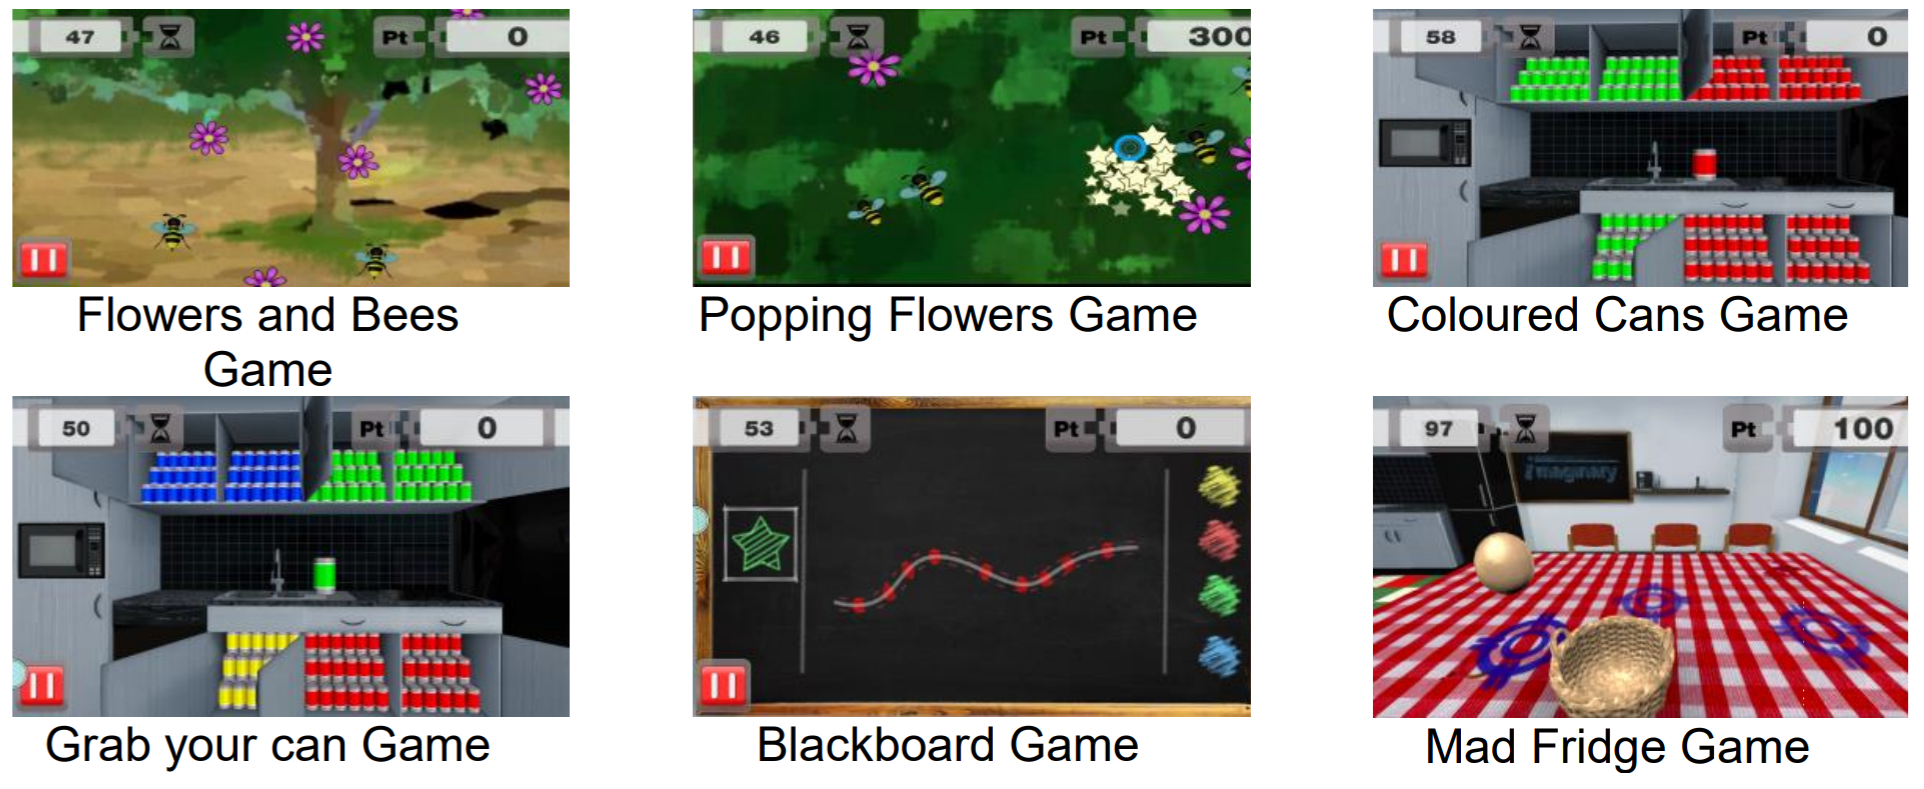
\includegraphics[width=1\linewidth]{figures/state_of_the_art/rehab@home}
	\caption{Spieleauswahl Rehab@Home \cite{figures:rehab@home:2016}}
	\label{fig:rehab@home:2016}
\end{figure}

\section{Gardener}\label{sec:gardener}
\enquote{Gardener} ist ein Serious Game für die Schlaganfallrehabilitation. Die Aufgabe des/der Spieler/in ist Pflanzen wachsen zu lassen. Um ein Gewächs sprießen zu lassen, muss der/die Patient/in dieses mit einer speziellen Geste gießen. Dieser Prozess kann solange wiederholt werden, bis alle Pflanzen im Garten ausgewachsen sind (siehe Abbildung \ref{fig:gardener}). Wenn eine Pflanze nicht gegossen wird, fängt sie an zu verwelken. Des Weiteren existiert Level-Editor, mit dem an diversen Stellschrauben des Spiels gedreht werden kann. Zum Beispiel kann die Anzahl der Pflanzen im Level verändert werden oder die Zeit, welche die Pflanzen benötigen, um zu verwelken. \cite{miesenberger:2014:gardener}

\begin{figure}[h]
    \centering
	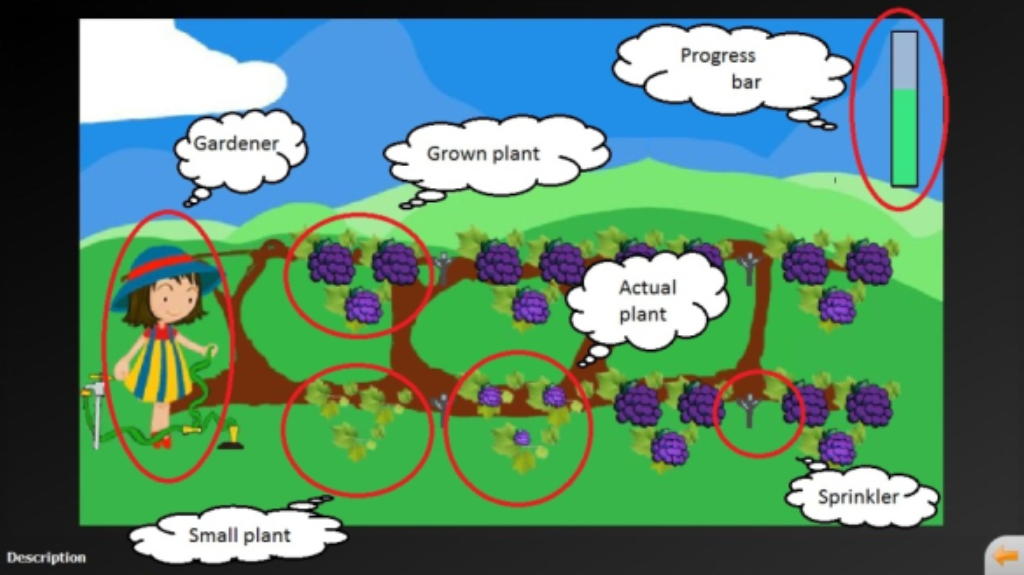
\includegraphics[width=0.8\linewidth]{figures/state_of_the_art/gardener}
	\caption{Ausschnitt aus Gardener \cite{miesenberger:2014:gardener}}
	\label{fig:gardener}
\end{figure}

%\section{Break the Bricks}
%\enquote{Break the Bricks} bezeichnet ein Serious Game für die Rehabilitation von Schlaganfallpatient/innen. Das Ziel des Spiels ist, dass alle Blöcke mithilfe eines abprallenden Balls zerstört werden müssen, während durch einen Block verhindert wird, dass der Ball durch den Boden fällt. Der Block wird mit der Bewegung des Telefons verschoben. Der/Die Patient/in wird durch das Absolvieren von diversen Leveln und dem Brechen von Highscores motiviert. Ein Vorteil des Spiels ist, dass es auf dem Beschleunigungssensor von Smartphones aufbaut, weswegen die Balancefähigkeit des/der Patient/in gefordert und geschult wird. Die genauen Armbewegungen sind Teil des Rehabilitationprozesses, da jene große Aufmerksamkeit benötigen.
%\cite{miesenberger:2012:computers}

\section{AGaR}\label{sec:agar}
Das Serious Game \enquote{AGaR} wurde mit der Technologie \ac{VR} vor allem für die Rehabilition des Oberkörpers von Schlaganfallpatient/innen entwickelt. Zur Interaktion mit dem Spiel kommt der Bewegungssensor Kinect One von Microsoft zum Einsatz. Das Hauptziel des Spiels ist es, dass Bilderpaare gefunden werden, die eine ähnliche oder eine komplementäre Bedeutung haben. Abbildung \ref{fig:agar} zeigt den hauptsächlichen Spielablauf. Es gibt ein Zielbild, von dem die entsprechende Bedeutung gefunden werden muss und vier selektierbare Darstellungen, aus denen eines gewählt werden kann. Um das Spiel zu gewinnen, muss das korrekte Bild auf das Zielbild gezogen werden. Die Anzahl der Wiederholungen gibt der/die Therapeut/in vor. Bevor mit der Auswahl begonnen werden kann, muss der/die Therapeut/in die Bewegung freigeben. Wenn ein falsches Bild gewählt wurde, kann der/die Behandelte das Bild, wie in Abbildung \ref{fig:agar} zu sehen ist, auf die Mülltonne ziehen, um die Auswahl zurückzusetzen. Wenn ein falsches Bild ausgewählt wurde, ertönt ein Geräusch, das den Fehler signalisiert  und danach verschwindet das Bild. Der/Die Patient/in kann anschließend aus den verbleibenden Bildern wählen. Um den Therapieerfolg zu messen, werden unter anderem folgende Daten für den/die Therapierende/n gespeichert: \cite{funabashi:agar:2017}

\begin{itemize}
	\item \textbf{Reaktionszeit}: Wie lange braucht der/die Patient/in, um den Cursor das erste Mal zu bewegen, nachdem die Bewegung freigegeben wurde.
	\item \textbf{Zeit um ein Bild zu wählen}: Wie lange braucht der/die Patient/in, um das erste Bild zu wählen, nachdem die Bewegung freigegeben wurde.
	\item \textbf{Verschiebzeit}: Wie lange hat es gedauert, bis der/die Patient/in das selektierte Bild auf das Zielbild geschoben hat. 
	\item \textbf{Spielzeit}: Wie lange hat das Spiel insgesamt gedauert.
\end{itemize}

\begin{figure}[h]
    \centering
	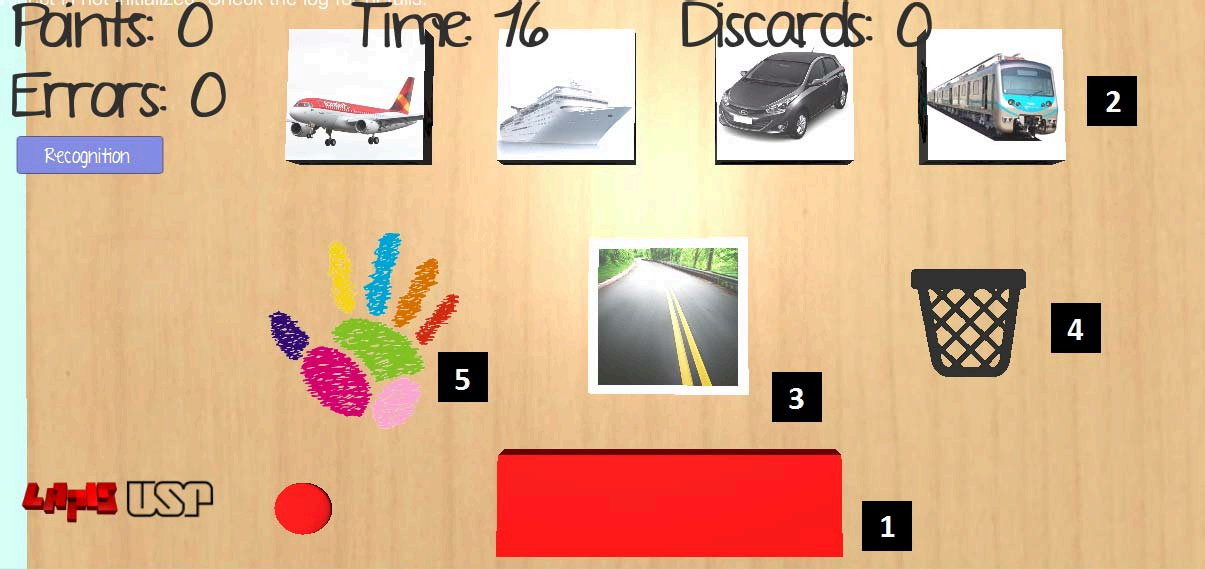
\includegraphics[width=0.8\linewidth]{figures/state_of_the_art/agar}
	\caption{Benutzeroberfläche von \enquote{AGaR}: Bereich 2 zeigt die auswählbaren Bilder, Bereich 3 zeigt das Zielbild, Bereich 4 dient dazu, die Auswahl zurückzusetzen, Bereich 5 stellt den Cursor des Patienten oder der Patient/in dar, der den Bewegungen über den Bildschirm folgt. \cite{funabashi:agar:2017}}
	\label{fig:agar}
\end{figure}

\section{RehaLabyrinth}\label{sec:reha-labyrinth}
\enquote{RehaLabyrinth} beschreibt ein Serious Game für die Rehabilitation von Schlaganfallpatient/innen, welches sich der Problematik annimmt, dass Betroffene nach einem Schlaganfall oft Probleme mit der Balance oder einer teilweisen Lähmung haben. Patient/innen fehlt oft die Motivation, wenn sie Therapieübungen zu Hause ausführen müssen. Das Serious Game setzt auf das Wii Fit Balance Board von Nintendo. Das Ziel des Spiels ist, dass ein weißer Ball durch ein Labyrinth ins Ziel navigiert werden muss (siehe Abbildung \ref{fig:reha_labyrinth}). Der/Die Anwender/in kontrolliert den Ball durch die Gewichtsverlagerung auf dem Balance Board. Der/Die Spieler/in kann zusätzlich noch Sterne sammeln, die als Bonuspunkte fungieren und in den Highscore einfließen. Darüber hinaus wird die Zeit, welche die Person zum Absolvieren des Levels benötigt, in die Bewertung miteinbezogen. Nachdem der/die Patient/in alle ausgewählten Levels absolviert hat, werden die Daten der Trainingssession persistent gespeichert und die Ergebnisse angezeigt. Außerdem existiert ein Level-Editor, der es erlaubt, die Level an die Bedürfnisse der behandelten Person anzupassen. Der/Die Therapierende hat pro Patient/in Zugriff auf Punktezahl, Zeit und die Kalibrierung des Wii Fit Balance Board. Zusätzlich wird noch die Bewegung der Patient/innen aufgezeichnet, die mit einem Referenzbewegungsmuster abgeglichen werden kann. Durch die Bewegungskurve kann der/die Therapeut/in eine halbseitige Lähmung feststellen. \cite{baranyi:reha_labyrinth:2013}

\begin{figure}[h]
    \centering
    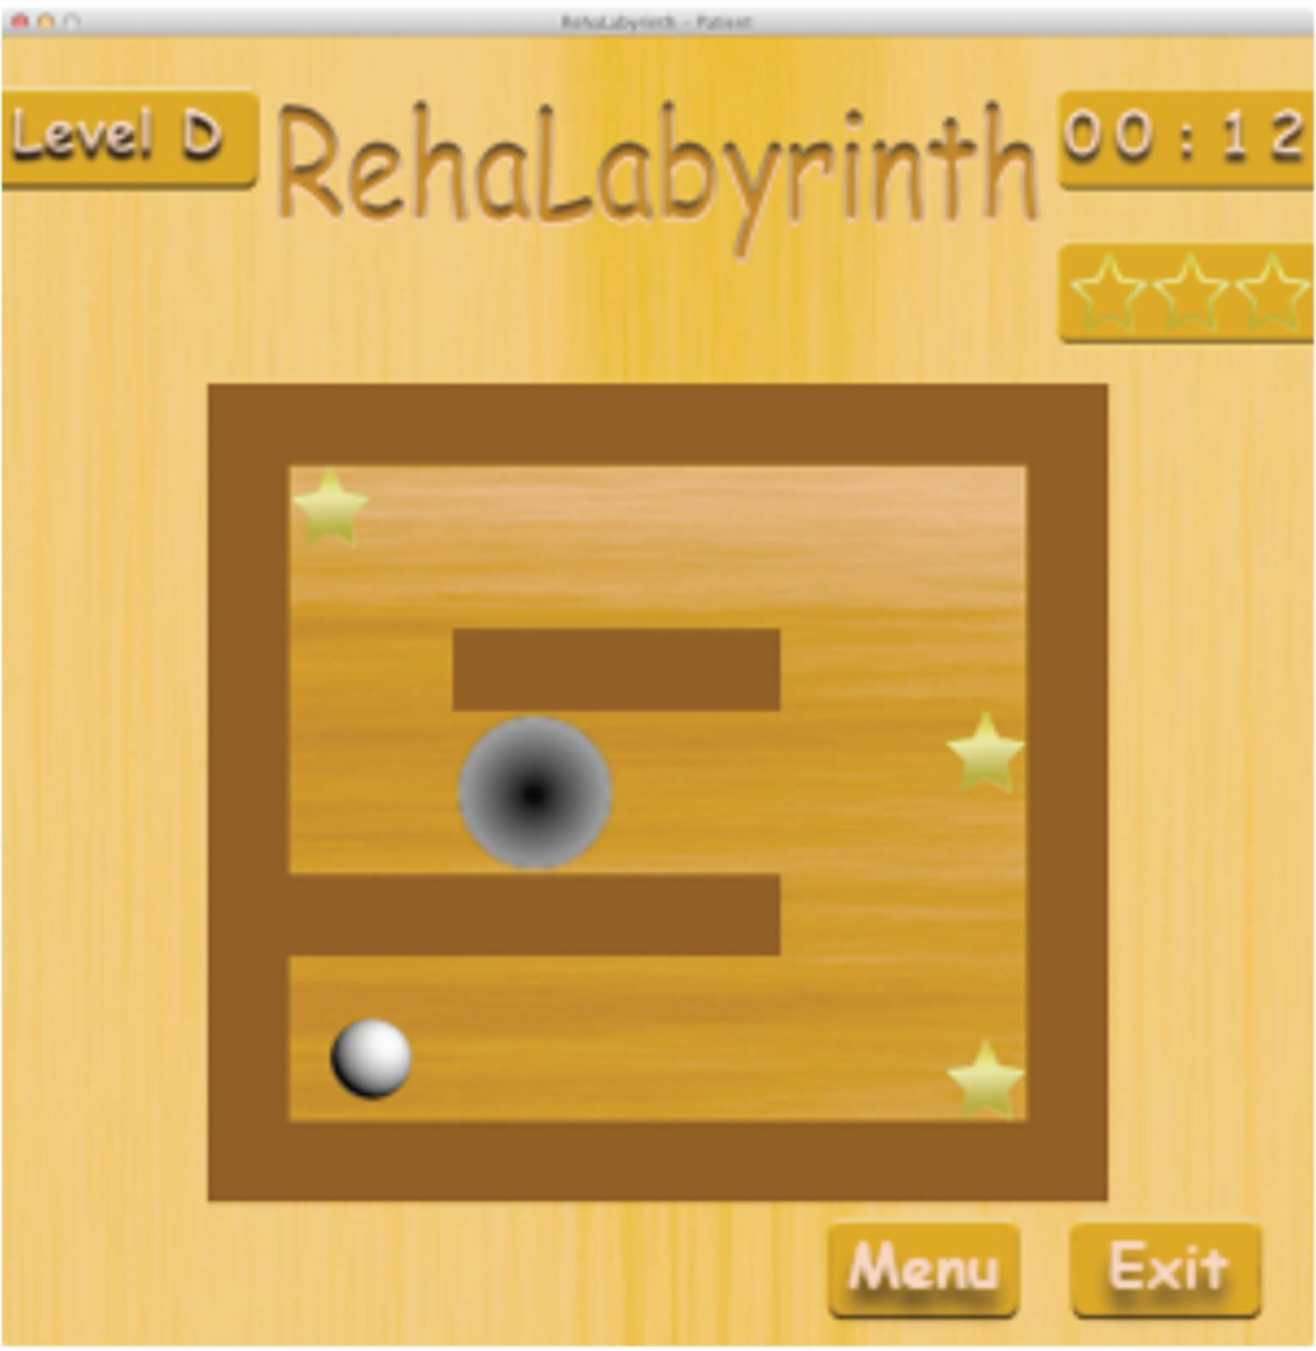
\includegraphics[width=0.6\linewidth]{figures/state_of_the_art/rehalabyrinth}
    \caption{Spielablauf aus \enquote{RehaLabyrinth} \cite{baranyi:reha_labyrinth:2013}}
    \label{fig:reha_labyrinth}
\end{figure}

\section{ROBiGame}\label{sec:robi-game}
\enquote{ROBiGame} bezeichnet ein Serious Game, dass speziell für die Verbesserung von motorischen und kognitiven Defiziten entwickelt wurde. Der Schwierigkeitsgrad des Spiels wird an die Performance des/der Patient/in angepasst. Als Hardware fungierte der REAplan End-Effektor Rehabilitationsroboter. So ein Roboter besteht üblicherweise aus einem horizontal beweglichen Griff, Kraft- und Positionssensoren, Motoren zur Unterstützung der Bewegung des Griffs und einem Bildschirm mit Lautsprechern. Das Thema des Spiels ist ein Sandwichgeschäft, wo der/die Patient/in Sandwiches zubereiten muss. Zu Beginn kommt ein/e Kund/in zum Laden und gibt eine Bestellung auf (siehe Abbildung \ref{fig:robigame}). Die Liste der Zutaten für die Bestellung wird neben dem/der Käufer/in angezeigt. Nachdem sich der/die Patient/in sich die Bestandteile des Sandwiches eingeprägt hat, kommt ein neues Fenster, wo der/die Betroffene den Auftrag aus den vorher angezeigten Zutaten zusammenbauen muss. Es gibt ein Zeitlimit, daher hat der Behandelte nicht unbegrenzt Zeit für die Zubereitung. Falls dieses abläuft, verlässt der/die Kundin wütend das Geschäft. Das Feedback für den/die Spieler/in wird durch Töne umgesetzt. Wenn eine falsche Zutat gegriffen wird, ertönt ein Fehlerton. Umgekehrt ertönt ein positiver Sound, wenn ein korrekter Bestandteil hinzugefügt wird. Am Ende einer Spielsitzung wird dem/der Patient/in angezeigt, wie viele Bestellungen korrekt abgearbeitet wurden. Die Fähigkeiten der behandelten Person werden durch eine Reihe von Variablen gemessen. Zu diesen Daten zählen: insgesamte Zeit der Durchführung, Griffpositionen im gesamten Spielverlauf, Krafteinwirkung auf den Griff und die motorische Unterstützung über die Zeit. Das Spiel wurde sehr positiv von den Patient/innen aufgenommen. \cite{heins:2017:robigame}

\begin{figure}[h]
    \centering
    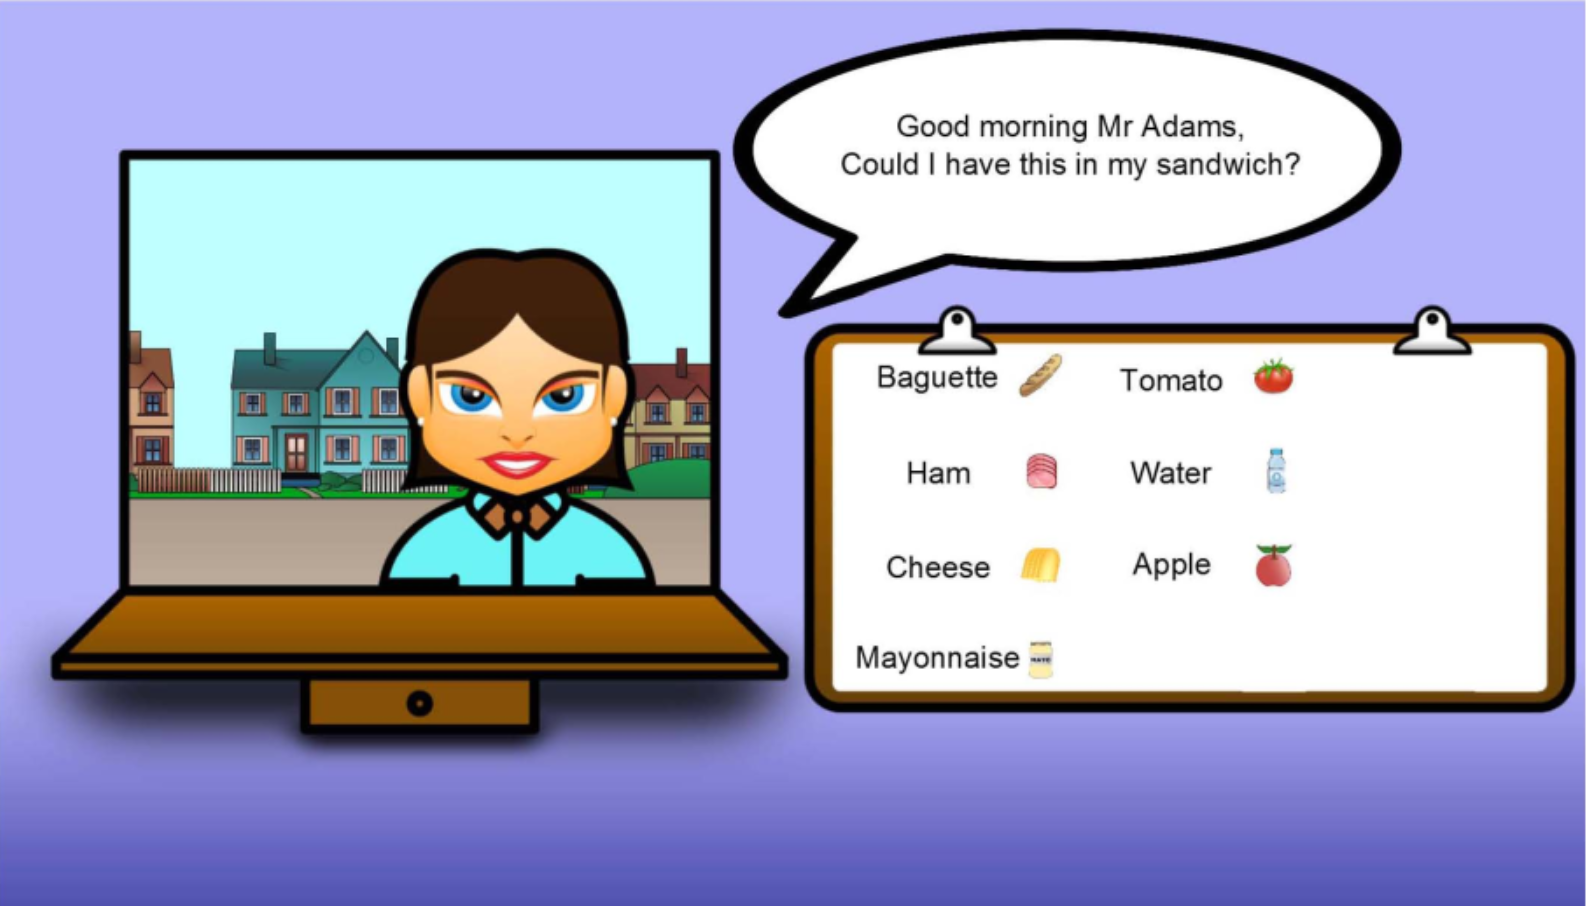
\includegraphics[width=0.7\linewidth]{figures/state_of_the_art/robigame}
    \caption{Illustration, wenn ein/e Kund/in ein Sandwich bestellt. Dieses Fenster erlaubt dem/der Partizipant/in einen ersten Überblick zu bekommen (\ac{z.B.}: Anzahl der Zutaten) \cite{heins:2017:robigame}}
    \label{fig:robigame}
\end{figure}

\section{Vergleich}
Diese Subkapitel vergleicht den entwickelten Prototypen namens \enquote{Plan your Day} mit anderen State of the Art Serious Games zur Behandlung von Patient/innen. In der Tabelle \ref{tab:serious-game-comparison} werden die unterschiedlichen Spiele anhand von einigen wichtigen Kriterien verglichen. Eines dieser Kriterien ist das Anwendungsgebiet der Applikation. Hier wird beschrieben, welche Fähigkeiten von der Anwendung trainiert werden. Weiters wird die Technologie, mit der die Anwendung bedient wird, beschrieben. Zudem ist noch wichtig, ob das Spiel theoretisch mit mehreren Spielern gleichzeitig gespielt werden kann. Feedback ist ein weiterer wichtiger Vergleichspunkt. Hier wird beschrieben, ob der/die Spieler/in akustische oder visuelle Rückmeldung bekommt. Des Weiteren wird verglichen, ob das Serious Game ausschließlich in einer medizinischen Einrichtung oder auch zu Hause verwendet werden kann. Das Kriterium \enquote{Kompetitiv} gibt an, ob Patient/innen ihre Ergebnisse, Highscores miteinander vergleichen können. Beim Punkt \enquote{Daten} wird erhoben, welche Informationen von den verschiedenen Anwendungen erhoben werden. Anpassbarkeit beschreibt, ob es den Therapierenden erlaubt ist, das Serious Game für ihre Patient/innen anzupassen.

\begin{table}[]
\begin{tabular}{|l|l|l|l|l|l|l|}
\hline
\rowcolor[HTML]{C0C0C0} 
\textbf{}                                                                        & \multicolumn{1}{c|}{\cellcolor[HTML]{C0C0C0}\textbf{\begin{tabular}[c]{@{}c@{}}Rehab@\\ Home\end{tabular}}} & \multicolumn{1}{c|}{\cellcolor[HTML]{C0C0C0}\textbf{Gardener}}                               & \multicolumn{1}{c|}{\cellcolor[HTML]{C0C0C0}\textbf{AGar}}                                                        & \textbf{\begin{tabular}[c]{@{}l@{}}Reha\\ Labyrinth\end{tabular}}     & \textbf{\begin{tabular}[c]{@{}l@{}}ROBi\\ Game\end{tabular}}                                                               & \textbf{\begin{tabular}[c]{@{}l@{}}Plan \\ your Day\end{tabular}}                                             \\ \hline
\textbf{\begin{tabular}[c]{@{}l@{}}Anwen-\\ dungs-\\ gebiet\end{tabular}}        & motorisch                                                                                                   & kognitiv                                                                                     & kognitiv                                                                                                          & motorisch                                                             & \begin{tabular}[c]{@{}l@{}}motorisch,\\ kognitiv\end{tabular}                                                              & \begin{tabular}[c]{@{}l@{}}kognititv, \\ exekutiv\end{tabular}                                                \\ \hline
\textbf{\begin{tabular}[c]{@{}l@{}}Interakti-\\ onstech-\\ nologie\end{tabular}} & \begin{tabular}[c]{@{}l@{}}Wii, \\ Kinect,\\ Stifteo- \\ Cubes\end{tabular}                                 & Tastatur                                                                                     & \begin{tabular}[c]{@{}l@{}}Kinect One,\\ VR\end{tabular}                                                          & \begin{tabular}[c]{@{}l@{}}Wii Fit \\ Balance\\ Board\end{tabular}    & \begin{tabular}[c]{@{}l@{}}REAplan \\ End-\\ Effektor\end{tabular}                                                         & \begin{tabular}[c]{@{}l@{}}Smart-\\ phone, \\ Tablet\end{tabular}                                             \\ \hline
\textbf{\begin{tabular}[c]{@{}l@{}}Spieler-\\ anzahl\end{tabular}}               & 1                                                                                                           & 1                                                                                            & 1                                                                                                                 & 1                                                                     & 1                                                                                                                          & 1                                                                                                             \\ \hline
\textbf{Feedback}                                                                & ja                                                                                                          & ja                                                                                           & ja                                                                                                                & ja                                                                    & ja                                                                                                                         & ja                                                                                                            \\ \hline
\textbf{\begin{tabular}[c]{@{}l@{}}Portier-\\ barkeit\end{tabular}}              & zu Hause                                                                                                    & -                                                                                            & Klink                                                                                                             & -                                                                     & Klinik                                                                                                                     & \begin{tabular}[c]{@{}l@{}}Klinik,\\ zu Hause\end{tabular}                                                    \\ \hline
\textbf{\begin{tabular}[c]{@{}l@{}}Kompe-\\ tetiv\end{tabular}}                  & ja                                                                                                          & nein                                                                                         & nein                                                                                                              & nein                                                                  & nein                                                                                                                       & nein                                                                                                          \\ \hline
\textbf{Daten}                                                                   & Punkte                                                                                                      & -                                                                                            & \begin{tabular}[c]{@{}l@{}}Reaktions-\\ zeit,\\ Spielzeit,\\ Verschiebe-\\ zeit,\\ Bildwähl-\\ zeit\end{tabular}  & \begin{tabular}[c]{@{}l@{}}Zeit,\\ Punkte,\end{tabular}               & \begin{tabular}[c]{@{}l@{}}Zeit,\\ Griff-\\ position,\\ Kraft-\\ einwirkung,\\ motorische\\ Unter-\\ stützung\end{tabular} & \begin{tabular}[c]{@{}l@{}}Fehler, \\ Zeit\end{tabular}                                                       \\ \hline
\textbf{\begin{tabular}[c]{@{}l@{}}Anpass-\\ bar\end{tabular}}                   & ja                                                                                                          & ja                                                                                           & ja                                                                                                                & ja                                                                    & ja                                                                                                                         & ja                                                                                                            \\ \hline
\textbf{Use case}                                                                & \begin{tabular}[c]{@{}l@{}}Auswahl\\ der \\ Spiele\\ durch\\ den/die\\ Ärzt/in\end{tabular}                 & \begin{tabular}[c]{@{}l@{}}Pflanzen\\ in \\ individu-\\ ellen\\ Leveln\\ gießen\end{tabular} & \begin{tabular}[c]{@{}l@{}}Bilder mit\\ ähnlicher \\ oder \\ komple-\\ mentärer\\ Bedeutung\\ finden\end{tabular} & \begin{tabular}[c]{@{}l@{}}Ball ins\\ Ziel \\ navigieren\end{tabular} & \begin{tabular}[c]{@{}l@{}}Einkaufsliste\\ abarbeiten\end{tabular}                                                         & \begin{tabular}[c]{@{}l@{}}Einkaufsliste\\ abarbeiten \\ nach\\ Konfiguration\\ durch\\ Therapeuten\end{tabular} \\ \hline
\end{tabular}
    \caption{Vergleich der State of the art Serious games.}
	\label{tab:serious-game-comparison}
\end{table}

Während andere Serious Games häufig mit Kinect, Wii-Balance Board oder eigener Hardware arbeiten, setzt \enquote{Plan your Day} auf die Eingabe mittels Smartphones oder Tablet. Durch diesen Umstand kann das Spiel einfach verbreitet werden und erreicht so die größtmögliche Spieler/innenanzahl. Das Spiel kann auch nach dem Aufenthalt in einer medizinischen Einrichtung weiter genutzt werden.